\chapter{Tehnologii utilizate}

În acest capitol sunt prezentate în primul rând tehnologiile utilizate în implementarea aplicației.

\section{Angular}
\begin{figure}[H]
	
\includegraphics[width=0.3\textwidth, left]{Angular-logo.png}
%	\caption{\url{https://www.vectorlogo.zone/logos/angular/angular-ar21.png}}
\end{figure}

\textbf{Angular} este un framework de JavaScript scris în TypeScript și menținut de Google. Framework-ul a fost dezvoltat în principal pentru crearea aplicațiilor web \textit{single-page}, într-o manieră ce ușurează mentenanța și dezvoltarea ulterioară.

\subsection{Scurt istoric}
În 2010, Miško Hevery, un angajat la Google la acel timp, a lansat un proiect cu numele \textit{AngularJS} care a fost apreciat în mare măsură de comunitate. Între anii 2014-2015 a avut loc o reîmprospăatare majoră a framework-ului însemnând de fapt o rescriere majoră a acestuia. Noua versiune avea să fie numită simplu Angular. Au urmat câțiva ani de tranziție deoarece multe proiecte deja în producție erau utilizau AngularJS și  trebuiau refactorizate. În acest moment, Angular este cel mai folosit framework de front-end, în specialde dezvoltatorii de la Google și de către start-up-uri. Exemple de companii recunoscute ce folosesc Angular sunt Microsoft, Gmail, PayPal, Forbes \cite{angular-history}.

\begin{figure}[H]
	\centering
	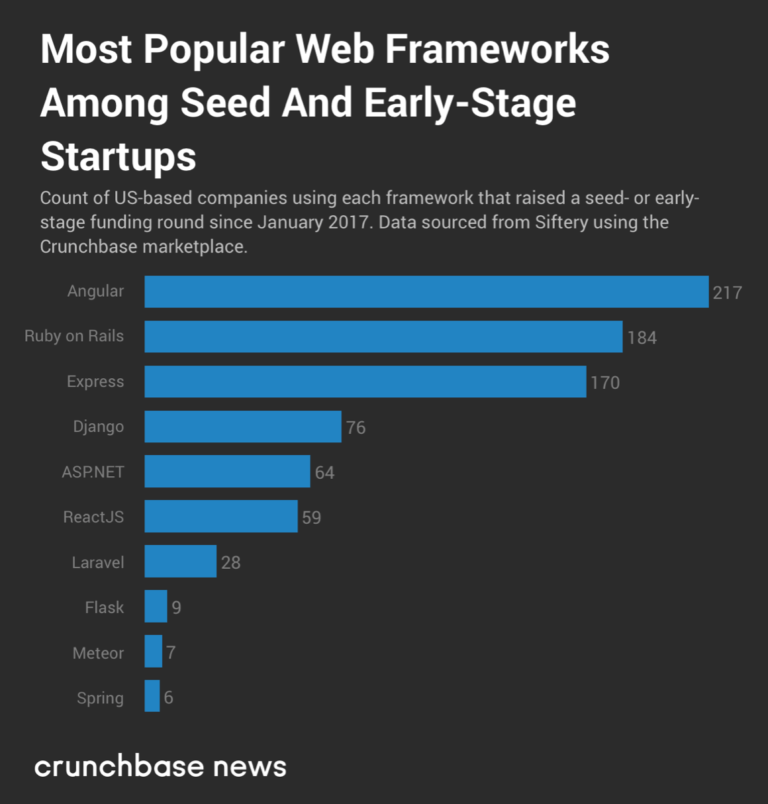
\includegraphics[width=0.8\textwidth]{Angular-crunchbase-newspng.png}
	\caption{\cite{angular-stats}}
\end{figure}

\subsection{Particularități}
Motivul alegerii Angular pe partea de front-end este reprezentat de o serie de caracteristici.

Un astfel de motiv este \textit{arhitectura bazată pe componente}, fiind astfel o formă de programare orientată pe obiect. Utilizatorul crează în mod uzual clase corespunzătoare componentelor ce conțin și un șablon HTML (\textit{eng.} HTML template). Pentru simplificare, Angular oferă și opțiunea de "injectare" a serviciilor \textit{custom} sau \textit{in-built} într-o componentă ce utilizează aceste funcționalități. În acest fel, utilizatorul poate reutiliza, înlocui, modifica componente în diverse locuri, obținându-se astfel un UI (User Interface) modularizat.

Un alt motiv este modul de încărcare a paginii web. Angular folosește \textit{lazy loading} ce permite încărcarea instantanee a website-urilor, prin afișarea doar a componentelor cerute și necesare utilizatorului, în timp ce celelalte sunt pregătite în fundal pentru alte eventualități.

\textit{Dependency injection} reprezintă un al treilea motiv, un design pattern ce permite împărțirea lucrului între diferite servicii, distribuind în mod eficient sarcinile. Prin inițializarea dependențelor, Angular reușește să reducă în mod considerabil codul de tip \textit{boilerplate} (fragmente similare de cod des utilizat între care există mici diferențe) și să extindă mai ușor o astfel de aplicație.

Framework-ul are trei tipuri de \textit{dependency injections}:
\begin{enumerate}
	\item Constructor injection
	\item Setter injection
	\item Interface injection
\end{enumerate}

Din punct de vedere al arhitecturii, Angular poate fi considerat în general un framework MVVM (Model-View-ViewModel), după cum se observă în figura următoare.

\begin{figure}[H]
	\centering
	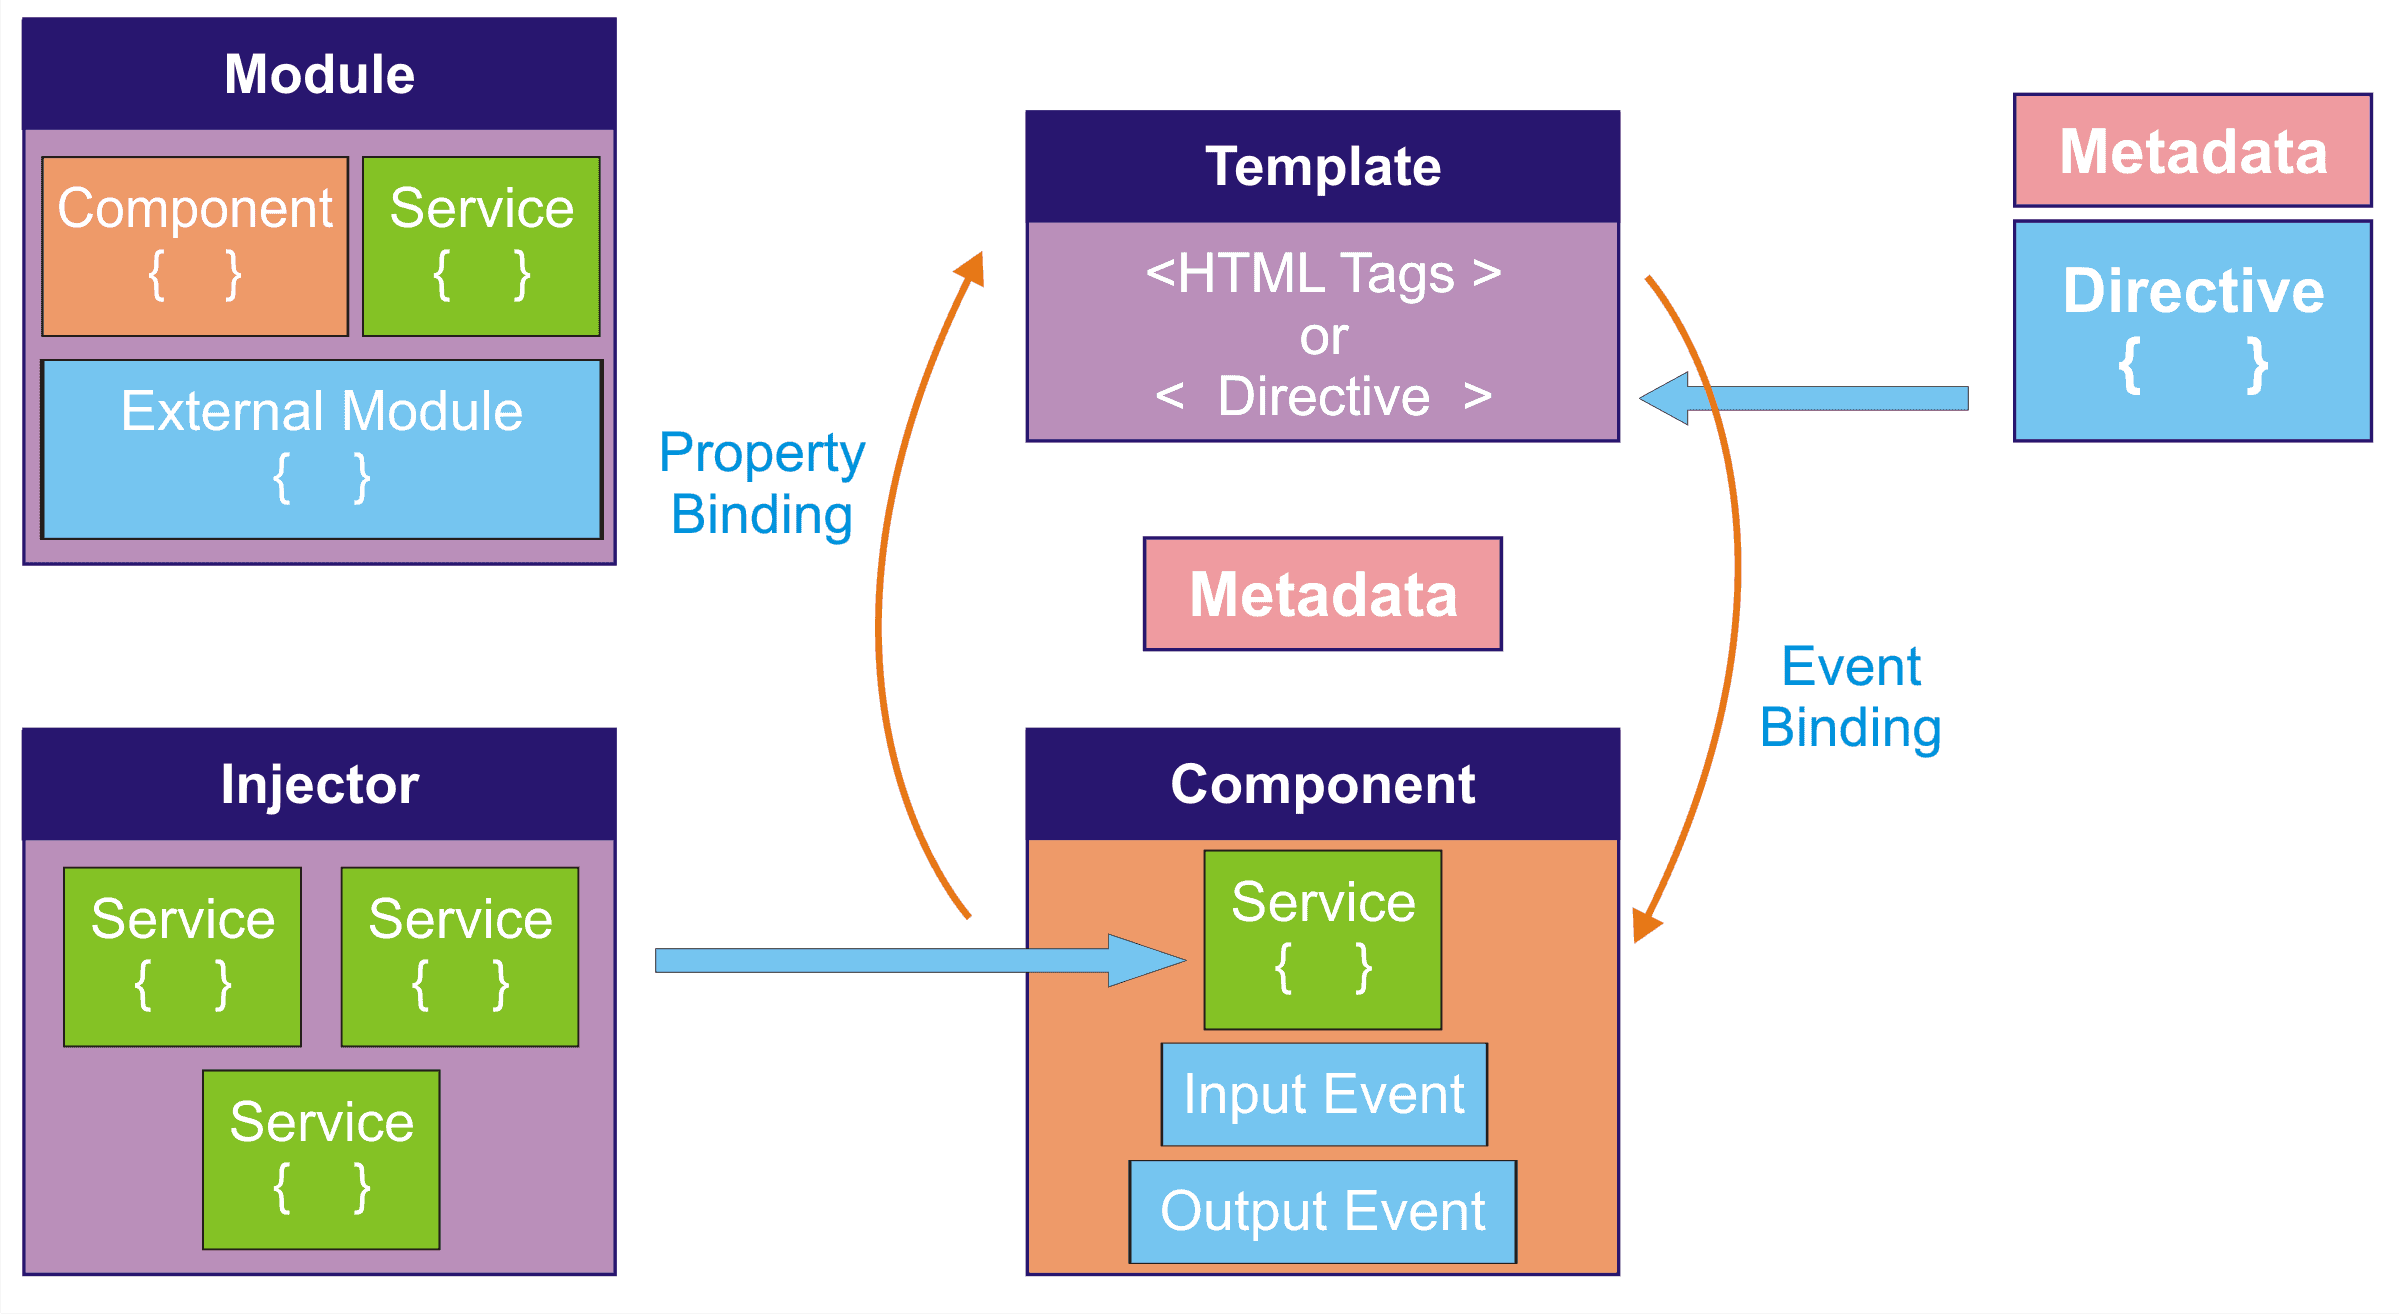
\includegraphics[width=0.6\textwidth]{Angular_Architecture.png}
	\caption{Arhitectura Angular \cite{angular-architecture-diagram}}
\end{figure}

\section{Spring Boot}
\begin{figure}[H]
	\centering
	
\includegraphics[width=0.3\textwidth, left]{Spring-boot-logo.jpg}
\end{figure}

\textbf{Spring Boot} este un micro-framework open-source folosit pentru a crea aplicații Spring cu microservicii. Spre deosebire de alte framework-uri de Java, acesta oferă configurări XML flexibile, 
procesare în loturi puternică, tranzacții cu baza de date și o varietate de instrumente de dezvoltare.

\subsection{Scurt istoric}
Framework-ul \textit{Spring} a fost creat în 2004 pentru a simplifica dezvoltarea programelor pe partea de server. În aprilie 2014 a fost lansat Spring boot 1.0.0 în urma unor cereri din partea programatorilor de a configura serviciile de web container într-un container spring din metoda principală. În decembrie 2016 a fost lansat Spring Boot 1.3 ulterior trecerii framework-ului Spring de la versiunea 4.1 la 4.2 și includea sprinjin pentru fisiere JAR complet executabile, noi utilitare spring-boot-dev și auto-configurare pentru tehnologii de caching. 

\subsection{Motivație}
Spring Boot este bazat pe Java, unul dintre cele mai populare limbaje de programare. Framework-ul are o comunitate vastă de utilizatori cu diverse materiale și cursuri.

\begin{figure}[H]
	\centering
	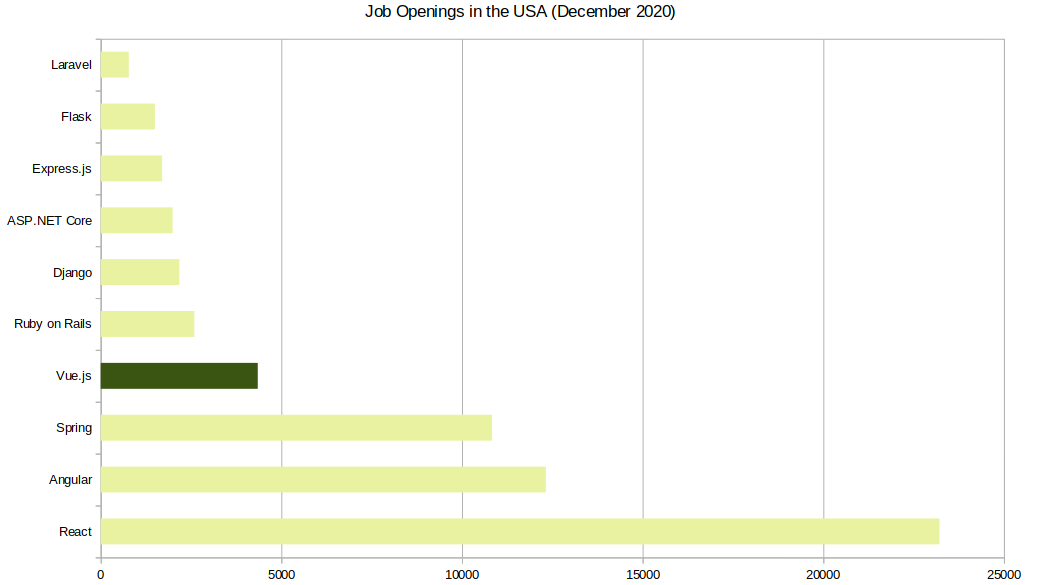
\includegraphics[width=0.6\textwidth]{Spring-ranking.png}
	\caption{\cite{spring-popularity}}
\end{figure}

Avantajele prinicipale sunt după cum urmează. Spring Boot este \textit{multi-threaded}, util pentru operații repetitive și de durată. Facilitează crearea și testarea aplicațiilor Java oferind un setup default pentru unit și integration testing. Există de asemenea posibilitatea de a integra Spring Boot cu ecosistemul Spring ce include Spring Data, Spring Security, Spring ORM și Spring JDBC într-un mod simplificat.

\subsection{Particularități}
Principala particularitate a Spring Boot o reprezintă adnotările (\textit{Spring Boot annotations}) utilizate în auto configurare.
De exemplu, \textbf{@SpringBootApplication} marchează metoda principală a aplicației și este obligatorie.
\textbf{@EnableAutoConfiguration} oferă oricărei clase pe care o marchează cu opțiunea de Automatic Configuration.
\textbf{@ComponentScan} scanează la inițializare toate declarările de \textit{beans} și pachete.

Un alt detaliu este utilizarea \textit{Spring Starter Dependencies} ce facilitează gestionarea dependențelor unei aplicații în continuă dezvoltare.

\textit{Spring Boot Actuator} oferă utilitare de producție aplicației. Actuator este utilizat în mare parte pentru a obține informații de funcționare despre o aplicație în rulare (metrice, info, dump, env, etc.), cu ajutorul HTTp endpoints și JMX beans.
Ultima versiune, Spring Boot 2.x Actuator, suportă și modele CRUD.

\subsection{Detalii}
Versiunea de Java este 11.

Versiunea de Spring Boot este 2.7.6.

\section{MySQL}

\begin{figure}[H]
	
\includegraphics[width=0.3\textwidth, left]{mysql-logo.png}
%	\caption{\url{https://download.logo.wine/logo/MySQL/MySQL-Logo.wine.png}}
\end{figure}

MySQL este cea mai populară bază de date open-source, fiind o soluție adoptată de aplicații des folosite precum Facebook, Twitter, Netflix \cite{about-mysql}. Este un sistem de gestionare a bazelor de date relaționale (RDMS) de tipul client/server care include un server SQL cu multiple fire de execuție (multi-threaded), diverse librării și API-uri.

\subsection{Avantaje}

MySQL este tehnologia aleasă pentru stocarea datelor datorită fiabilității și scalabilității sale, precum și funcționalităților variate. De asemenea, integrarea cu alte tehnologii precum Spring Boot are loc ușor datorită librăriilor și soluțiilor unei comunități extinse de utilizatori.

A fost aleasă o bază de date relațională pentru a asigura consistența datelor, luând în calcul numărul mare de preferințe al studenților ce trebuie procesate.